% =====================================================================
%  ملف الشرح – التجربة 9: طرق التشغيل والكبح للمحرك اللاتزامني
%  مساعدة شخصية (ليست للتسليم) – النسخة العربية
%  الترجمة: xelatex erklaerung_ar.tex (مرتين)
% =====================================================================
\documentclass[11pt,a4paper]{article}
\usepackage[a4paper,left=2.3cm,right=2.3cm,top=2.5cm,bottom=2.5cm]{geometry}
\usepackage{amsmath,amssymb}
\usepackage[locale=DE,per-mode=symbol]{siunitx}
\usepackage{graphicx}
\usepackage{booktabs}
\usepackage{array}
\usepackage{float}
\usepackage{enumitem}
\setlist{itemsep=2pt,topsep=4pt}
\usepackage{xcolor}
\usepackage[most]{tcolorbox}
\usepackage{fancyhdr}
\usepackage[colorlinks=true,linkcolor=black,urlcolor=blue!50!black]{hyperref}
\usepackage{polyglossia}
\setmainlanguage[numerals=maghrib]{arabic}
\setotherlanguage{german}
\setmainfont{Latin Modern Roman}
\newfontfamily\arabicfont[Script=Arabic,Scale=1.15]{Amiri}
\newfontfamily\arabicfontsf[Script=Arabic,Scale=1.15]{Amiri}
\newfontfamily\arabicfonttt[Script=Arabic,Scale=1.15]{Amiri}

\graphicspath{{../bericht/abbildungen/}}
% automatisch erzeugt von auswertung/auswertung.py
\newcommand{\WJStahl}{0{,}3711}
\newcommand{\WJAlu}{0{,}1277}
\newcommand{\WJVorb}{0{,}3745}
\newcommand{\WdtBsp}{42{,}6}
\newcommand{\WtHDA}{1{,}20}
\newcommand{\WtHDB}{1{,}29}
\newcommand{\WtHDC}{1{,}40}
\newcommand{\WtHYA}{3{,}62}
\newcommand{\WtHYB}{3{,}92}
\newcommand{\WtHYC}{4{,}24}
\newcommand{\WdirektIeins}{50{,}66}
\newcommand{\WdirektUnull}{405}
\newcommand{\WdirektUeins}{388}
\newcommand{\WdirektPeins}{17896}
\newcommand{\WdirektQeins}{56162}
\newcommand{\Wdirektnend}{1499}
\newcommand{\WdirektIend}{4{,}58}
\newcommand{\WdirektPend}{1747}
\newcommand{\WdirektQend}{5175}
\newcommand{\Wdirekttneunacht}{1{,}14}
\newcommand{\Wdirektteinsvierfuenfnull}{1{,}10}
\newcommand{\WdirektE}{14509}
\newcommand{\WdirektdU}{4{,}3}
\newcommand{\WdirektIfak}{11{,}0}
\newcommand{\WdirektIN}{7{,}6}
\newcommand{\WfruehIeins}{15{,}51}
\newcommand{\WfruehUnull}{405}
\newcommand{\WfruehUeins}{400}
\newcommand{\WfruehPeins}{6685}
\newcommand{\WfruehQeins}{17788}
\newcommand{\Wfruehnend}{1497}
\newcommand{\WfruehIend}{4{,}59}
\newcommand{\WfruehPend}{1760}
\newcommand{\WfruehQend}{5173}
\newcommand{\Wfruehtneunacht}{2{,}65}
\newcommand{\Wfruehteinsvierfuenfnull}{2{,}62}
\newcommand{\WfruehE}{15389}
\newcommand{\WfruehdU}{1{,}2}
\newcommand{\WfruehIfak}{3{,}4}
\newcommand{\WfruehIN}{2{,}3}
\newcommand{\Wfruehtum}{1{,}91}
\newcommand{\Wfruehnum}{724}
\newcommand{\Wfruehpause}{0{,}16}
\newcommand{\WfruehIzwei}{45{,}91}
\newcommand{\WfruehUzwei}{384}
\newcommand{\WfruehPzwei}{20422}
\newcommand{\WfruehdUzwei}{5{,}1}
\newcommand{\WrichtigIeins}{15{,}51}
\newcommand{\WrichtigUnull}{405}
\newcommand{\WrichtigUeins}{400}
\newcommand{\WrichtigPeins}{5635}
\newcommand{\WrichtigQeins}{17779}
\newcommand{\Wrichtignend}{1497}
\newcommand{\WrichtigIend}{4{,}57}
\newcommand{\WrichtigPend}{1755}
\newcommand{\WrichtigQend}{5162}
\newcommand{\Wrichtigtneunacht}{3{,}86}
\newcommand{\Wrichtigteinsvierfuenfnull}{3{,}82}
\newcommand{\WrichtigE}{15754}
\newcommand{\WrichtigdU}{1{,}3}
\newcommand{\WrichtigIfak}{3{,}4}
\newcommand{\WrichtigIN}{2{,}3}
\newcommand{\Wrichtigtum}{3{,}60}
\newcommand{\Wrichtignum}{1443}
\newcommand{\Wrichtigpause}{0{,}14}
\newcommand{\WrichtigIzwei}{42{,}25}
\newcommand{\WrichtigUzwei}{402}
\newcommand{\WrichtigPzwei}{11284}
\newcommand{\WrichtigdUzwei}{0{,}9}
\newcommand{\WfalschIeins}{15{,}71}
\newcommand{\WfalschUnull}{405}
\newcommand{\WfalschUeins}{400}
\newcommand{\WfalschPeins}{5622}
\newcommand{\WfalschQeins}{18202}
\newcommand{\Wfalschnend}{1498}
\newcommand{\WfalschIend}{4{,}58}
\newcommand{\WfalschPend}{1781}
\newcommand{\WfalschQend}{5172}
\newcommand{\Wfalschtneunacht}{3{,}90}
\newcommand{\Wfalschteinsvierfuenfnull}{3{,}59}
\newcommand{\WfalschE}{15842}
\newcommand{\WfalschdU}{1{,}3}
\newcommand{\WfalschIfak}{3{,}4}
\newcommand{\WfalschIN}{2{,}4}
\newcommand{\Wfalschtum}{3{,}62}
\newcommand{\Wfalschnum}{1453}
\newcommand{\Wfalschpause}{0{,}15}
\newcommand{\WfalschIzwei}{50{,}91}
\newcommand{\WfalschUzwei}{401}
\newcommand{\WfalschPzwei}{19180}
\newcommand{\WfalschdUzwei}{1{,}0}
\newcommand{\WtHYum}{3{,}87}
\newcommand{\WdirektMBmittel}{52{,}7}
\newcommand{\WfruehMBmittel}{14{,}8}
\newcommand{\WrichtigMBmittel}{15{,}8}
\newcommand{\WfalschMBmittel}{15{,}9}
\newcommand{\WMkennDmittel}{48{,}8}
\newcommand{\WMkennYmittel}{16{,}1}
\newcommand{\WEkin}{2268}
\newcommand{\Wfedernnull}{1801}
\newcommand{\WfedertB}{0{,}88}
\newcommand{\Wfederts}{0{,}12}
\newcommand{\WfederMmit}{31{,}7}
\newcommand{\WfederMmax}{32{,}0}
\newcommand{\WfederUzkmax}{583}
\newcommand{\WfederErb}{0}
\newcommand{\Wfederverz}{2047}
\newcommand{\Wfedernullnnull}{1801}
\newcommand{\WfedernulltB}{0{,}90}
\newcommand{\Wfedernullts}{0{,}12}
\newcommand{\WfedernullMmit}{30{,}8}
\newcommand{\WfedernullMmax}{31{,}3}
\newcommand{\WfedernullUzkmax}{583}
\newcommand{\WfedernullErb}{0}
\newcommand{\Wfedernullverz}{1996}
\newcommand{\WdclnI}{1773}
\newcommand{\WdclIdcB}{14{,}1}
\newcommand{\WdclIeffB}{9{,}4}
\newcommand{\WdcltI}{1{,}03}
\newcommand{\WdcltnachI}{5{,}17}
\newcommand{\Wdclnnull}{1801}
\newcommand{\WdcltB}{6{,}20}
\newcommand{\Wdclts}{0{,}40}
\newcommand{\WdclMmit}{4{,}6}
\newcommand{\WdclMmax}{21{,}4}
\newcommand{\WdclUzkmax}{595}
\newcommand{\WdclErb}{0}
\newcommand{\Wdclverz}{290}
\newcommand{\WdcmnI}{1774}
\newcommand{\WdcmIdcB}{20{,}5}
\newcommand{\WdcmIeffB}{13{,}7}
\newcommand{\WdcmtI}{1{,}02}
\newcommand{\WdcmtnachI}{2{,}43}
\newcommand{\Wdcmnnull}{1801}
\newcommand{\WdcmtB}{3{,}45}
\newcommand{\Wdcmts}{0{,}41}
\newcommand{\WdcmMmit}{9{,}7}
\newcommand{\WdcmMmax}{33{,}9}
\newcommand{\WdcmUzkmax}{596}
\newcommand{\WdcmErb}{0}
\newcommand{\Wdcmverz}{521}
\newcommand{\WdcsnI}{1774}
\newcommand{\WdcsIdcB}{32{,}8}
\newcommand{\WdcsIeffB}{21{,}9}
\newcommand{\WdcstI}{1{,}03}
\newcommand{\WdcstnachI}{0{,}95}
\newcommand{\Wdcsnnull}{1801}
\newcommand{\WdcstB}{1{,}98}
\newcommand{\Wdcsts}{0{,}42}
\newcommand{\WdcsMmit}{25{,}5}
\newcommand{\WdcsMmax}{57{,}5}
\newcommand{\WdcsUzkmax}{596}
\newcommand{\WdcsErb}{0}
\newcommand{\Wdcsverz}{929}
\newcommand{\Wgenohnennull}{1801}
\newcommand{\WgenohnetB}{8{,}49}
\newcommand{\Wgenohnets}{0{,}09}
\newcommand{\WgenohneMmit}{2{,}9}
\newcommand{\WgenohneMmax}{19{,}6}
\newcommand{\WgenohneUzkmax}{815}
\newcommand{\WgenohneErb}{0}
\newcommand{\Wgenohneverz}{211}
\newcommand{\Wgenlnnull}{1801}
\newcommand{\WgenltB}{10{,}12}
\newcommand{\Wgenlts}{0{,}14}
\newcommand{\WgenlMmit}{2{,}4}
\newcommand{\WgenlMmax}{2{,}8}
\newcommand{\WgenlUzkmax}{724}
\newcommand{\WgenlErb}{512}
\newcommand{\Wgenlverz}{177}
\newcommand{\Wgenmnnull}{1801}
\newcommand{\WgenmtB}{5{,}13}
\newcommand{\Wgenmts}{0{,}10}
\newcommand{\WgenmMmit}{4{,}8}
\newcommand{\WgenmMmax}{5{,}8}
\newcommand{\WgenmUzkmax}{724}
\newcommand{\WgenmErb}{1365}
\newcommand{\Wgenmverz}{349}
\newcommand{\Wgensnnull}{1801}
\newcommand{\WgenstB}{0{,}87}
\newcommand{\Wgensts}{0{,}06}
\newcommand{\WgensMmit}{29{,}6}
\newcommand{\WgensMmax}{39{,}2}
\newcommand{\WgensUzkmax}{723}
\newcommand{\WgensErb}{1821}
\newcommand{\Wgensverz}{2061}
\newcommand{\WRb}{28}
\newcommand{\WPRbmax}{7760}
\newcommand{\WgensErbAnteil}{80}


\newtcolorbox{merke}{colback=green!5,colframe=green!45!black,fonttitle=\bfseries,
  title={تذكّر},boxrule=0.6pt,arc=1mm}
\newtcolorbox{einfach}{colback=yellow!7,colframe=orange!70!black,fonttitle=\bfseries,
  title={شرح مبسّط},boxrule=0.6pt,arc=1mm}
\newtcolorbox{frage}[1]{colback=blue!4,colframe=blue!50!black,fonttitle=\bfseries,
  title={#1},boxrule=0.6pt,arc=1mm}
\newtcolorbox{achtung}{colback=red!4,colframe=red!60!black,fonttitle=\bfseries,
  title={انتبه / تحقّق بنفسك},boxrule=0.6pt,arc=1mm}
% مصطلح ألماني بين قوسين
\newcommand{\de}[1]{(\textgerman{\itshape #1})}
\newcommand{\dt}[1]{\textgerman{#1}}
\newcommand{\datei}[1]{\textgerman{\texttt{#1}}}

\pagestyle{fancy}\fancyhf{}
\fancyhead[R]{ملف الشرح – التجربة 9}\fancyhead[L]{\textgerman{Versuch 9}}
\fancyfoot[C]{\thepage}

\begin{document}
\sloppy
\begin{center}
{\LARGE\bfseries ملف الشرح – التجربة 9}\\[4pt]
{\Large طرق التشغيل والكبح للمحرك اللاتزامني}\\[2pt]
{\normalsize\dt{(Versuch 9: Anlauf- und Bremsverfahren)}}\\[6pt]
{\normalsize كل نقاط التجربة مشروحة خطوة بخطوة – للفهم والمذاكرة والتحضير للامتحان الشفهي \de{Testat}}
\end{center}

\begin{achtung}
التقرير والرسوم البيانية باللغة الألمانية، كما في المختبر. لذلك نكتب المصطلحات الألمانية المهمة
بين قوسين. في آخر الملف (القسم~\ref{sec:lexique}) يوجد قاموس صغير يترجم الكلمات المكتوبة على الرسوم.
\end{achtung}

\tableofcontents
\newpage

% =====================================================================
\section{عن ماذا تتحدث التجربة؟ (الخيط الأحمر)}
% =====================================================================
للتجربة جزءان:
\begin{enumerate}
\item \textbf{التشغيل} \de{Anlauf}: كيف نشغّل محركًا لاتزامنيًا دون أن نُحمّل الشبكة الكهربائية كثيرًا؟
  نقارن \emph{التشغيل المباشر بتوصيلة المثلث} \de{direkter Dreieckanlauf}
  مع \emph{التشغيل نجمة-مثلث} \de{Stern-Dreieck-Anlauf}.
  وقبل التجربة نحسب مدة التسارع.
\item \textbf{الكبح} \de{Bremsen}: كيف نوقف محركًا يدور مع حذافة بسرعة؟
  نقارن \emph{فرامل النابض} \de{Federkraftbremse}، و\emph{الكبح بالتيار المستمر} \de{DC-Bremse}،
  و\emph{الكبح التوليدي} \de{generatorisches Bremsen} مع مقاومة كبح \de{Bremswiderstand} وبدونها.
\end{enumerate}
المعادلة الوحيدة التي تربط كل شيء هي \textbf{معادلة الحركة} \de{Bewegungsgleichung}:
\[
  J\cdot\frac{\mathrm d\omega}{\mathrm dt} = M_\mathrm{Motor} - M_\mathrm{Last}.
\]
\begin{einfach}
العزم يُسرّع أو يُبطئ كتلة دوّارة، تمامًا كما تُسرّع القوة سيارة أو تُبطئها ($F = m\cdot a$).
هنا: $M = J\cdot\alpha$
\begin{itemize}
\item $J$ هو «الكتلة في الدوران» (عزم القصور الذاتي، بوحدة \si{kg.m^2})،
\item $\alpha = \mathrm d\omega/\mathrm dt$ هو التسارع الزاوي.
\end{itemize}
بهذه المعادلة يمكنك الحساب \emph{في الاتجاهين}:
\begin{itemize}
\item العزم معروف $\Leftarrow$ نحسب الزمن (التحضير، زمن التسارع).
\item السرعة مقيسة $\Leftarrow$ نحسب العزم (تقييم القياسات).
\end{itemize}
\end{einfach}

% =====================================================================
\section{الأساسيات التي يجب أن تفهمها}
% =====================================================================
\subsection{لماذا تيار التشغيل كبير جدًا؟}
المحرك اللاتزامني وهو متوقف يشبه \textbf{محولًا ملفه الثانوي في حالة قصر}:
قفص الدوّار حلقة مقصورة. عند التوقف (الانزلاق $s=1$) يمرّ مجال الجزء الثابت بكامل سرعته أمام الدوّار،
فيُحَث جهد كبير ويمرّ تيار كبير. لا يحدّه إلا ممانعة القصر الصغيرة.

\textbf{الانزلاق} \de{Schlupf}: $s = \dfrac{n_s - n}{n_s}$، حيث $n_s = \dfrac{f}{p}$ هي السرعة التزامنية.
عند \SI{50}{Hz} و $p=2$: $n_s = \SI{1500}{\per\minute}$.
\begin{itemize}
\item عند التوقف: $s=1$، تيار كبير.
\item عند السرعة الاسمية \SI{1420}{\per\minute}: $s\approx 0{,}05$، تيار صغير.
\end{itemize}
\textbf{المقيس:} في التشغيل المباشر \SI{\WdirektIeins}{A}، أي \WdirektIN{} ضعف التيار الاسمي
\SI{6,65}{A}. وهذا ضمن المجال المعروف في الكتب (من 5 إلى 8 أضعاف).

\subsection{لماذا ينخفض جهد الشبكة؟}
للشبكة (المحول والكابلات) ممانعة داخلية $Z_k = R_k + \mathrm jX_k$.
عندما يمرّ تيار كبير يسقط جزء من الجهد عليها، فيصل إلى المحرك جهد أقل.

\textbf{لماذا يكون الانخفاض قويًا عند التشغيل بالذات؟}
\begin{itemize}
\item تيار التشغيل تقريبًا تيار ردّي (غير فعّال) خالص (المقيس: $\cos\varphi\approx0{,}3$).
\item في المحول تكون $X_k$ أكبر بكثير من $R_k$.
\item لذلك يكون هبوط الجهد $\mathrm jX_k\cdot I$ موازيًا تقريبًا لجهد الشبكة فيُنقصه مباشرة.
\end{itemize}
هذا هو \textbf{مثلث كاب} \de{Kapp'sches Dreieck}:
$\Delta U \approx I\,(R_k\cos\varphi + X_k\sin\varphi)$.
وعندما $\sin\varphi\approx1$ تؤثر القيمة الكاملة $X_k\cdot I$.

\subsection{النجمة والمثلث – المعاملان \texorpdfstring{$\sqrt3$}{جذر 3} و 3}
\begin{center}
\begin{tabular}{@{}lcc@{}}
\toprule
& نجمة \dt{(Y)} & مثلث \dt{($\Delta$)}\\
\midrule
الجهد على ملف الطور & $400/\sqrt3 = \SI{230}{V}$ & \SI{400}{V}\\
تيار ملف الطور & $\frac{1}{\sqrt3}\cdot I_{\mathrm{Str},\Delta}$ & $I_{\mathrm{Str},\Delta}$\\
تيار الخط (الشبكة) & $\frac13\cdot I_{\mathrm{Netz},\Delta}$ & $I_{\mathrm{Netz},\Delta} = \sqrt3\,I_{\mathrm{Str},\Delta}$\\
العزم ($\sim U^2$) & $\frac13\cdot M_\Delta$ & $M_\Delta$\\
\bottomrule
\end{tabular}
\end{center}
\textbf{من أين يأتي المعامل 3 في تيار الخط؟}
\begin{itemize}
\item في النجمة يكون جهد الملف أصغر بـ $\sqrt3$، فيصغر تيار الملف بنفس النسبة.
\item في المثلث يكون تيار الخط أكبر من تيار الملف بـ $\sqrt3$ إضافية.
\item معًا: $\sqrt3\cdot\sqrt3 = 3$.
\end{itemize}
\textbf{المقيس:} $\WdirektIeins/\WrichtigIeins\approx 3{,}3$، وهذا مطابق جيدًا.

\textbf{لماذا $M\sim U^2$؟} الفيض يتناسب مع $U$، وتيار الدوّار أيضًا يتناسب مع $U$.
العزم = الفيض × التيار، إذن يتناسب مع $U^2$.

\begin{merke}
توصيلة نجمة-مثلث تُخفّض التيار \emph{و}العزم إلى الثلث. لذلك لا تنجح إلا إذا كان الحِمل عند
التشغيل صغيرًا (مراوح، مضخات، حذافة بلا حمل). أما السيور الناقلة أو الرافعات المُحمّلة فثلث العزم
غالبًا لا يكفيها.
\end{merke}

\subsection{منحنى العزم \texorpdfstring{$M(n)$}{M(n)}}
نقاط مهمة (انظر الشكل~\ref{fig:kenn}):
\begin{itemize}
\item \textbf{عزم البدء} \de{Anzugsmoment} عند $n=0$: هنا \SI{46}{Nm}.
\item \textbf{عزم السَّرج} \de{Sattelmoment}: انخفاض صغير عند حوالي \SI{200}{\per\minute}.
      سببه التوافقيات، وهو معتاد في الدوّارات القفصية.
\item \textbf{عزم الانقلاب} \de{Kippmoment}، أي القيمة العظمى: حوالي \SI{56}{Nm} عند \SI{1000}{\per\minute}.
\item بعده ينخفض العزم بشدة ويصبح صفرًا عند $n_s = \SI{1500}{\per\minute}$.
      بدون انزلاق لا يُحَث شيء، فلا يوجد عزم.
\end{itemize}
\begin{figure}[H]\centering
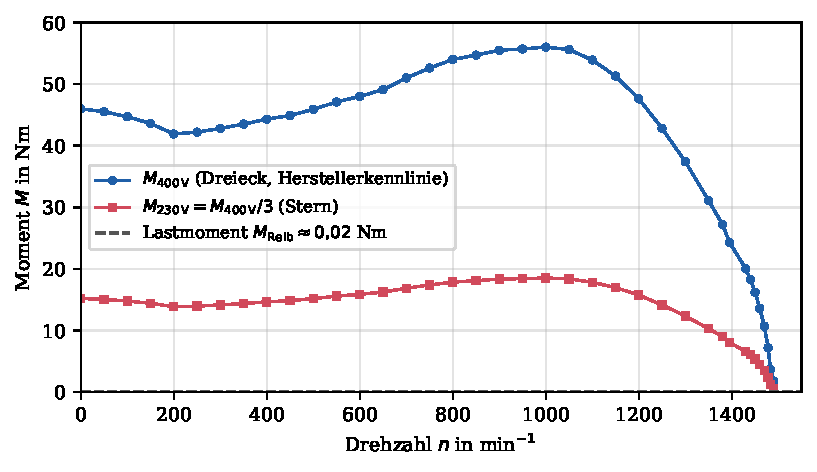
\includegraphics[width=0.8\textwidth]{v_kennlinie}
\caption{منحنى العزم (مقروء من دليل التجربة) ومنحنى النجمة (الثلث)}
\label{fig:kenn}
\end{figure}

\subsection{عزم القصور الذاتي \texorpdfstring{$J$}{J}}
لقرص مصمت: $J = \frac12 m r^2$، حيث نصف القطر $r = d/2 = \SI{0,15}{m}$.
\begin{itemize}
\item القرص الفولاذي (التشغيل): $J = 0{,}5\cdot32{,}99\cdot0{,}15^2 = \SI{\WJStahl}{kg.m^2}$.
\item قرص الألمنيوم (الكبح): $J = 0{,}5\cdot11{,}35\cdot0{,}15^2 = \SI{\WJAlu}{kg.m^2}$.
\item الدليل يذكر \SI{0,3745}{kg.m^2}. هذا أكثر قليلًا من القرص الفولاذي وحده،
      والأرجح أن عزم قصور دوّار المحرك محسوب معه.
\end{itemize}

% =====================================================================
\section{التحضير: حساب زمن التسارع خطوة بخطوة}
% =====================================================================
\textbf{الفكرة:} نقسم مجال السرعة إلى قطع صغيرة (مثلًا كل \SI{50}{\per\minute}).
في كل قطعة نعتبر العزم ثابتًا ونحسب كم تستغرق. في النهاية نجمع كل الأزمنة.
هذا يسمى \textbf{التكامل العددي}.

\textbf{اشتقاق المعادلة:}
\begin{align*}
J\,\frac{\Delta\omega}{\Delta t} &= M
\quad\Rightarrow\quad \Delta t = \frac{J\,\Delta\omega}{M},
\qquad \Delta\omega = 2\pi\,\Delta n\;(\Delta n \text{ in } \si{\per\second})\\
\Rightarrow\quad \Delta t &= \frac{2\pi\,J\,\Delta n}{M}.
\end{align*}

\textbf{مثال} للخطوة الأولى من 0 إلى \SI{50}{\per\minute} في المثلث:
\begin{enumerate}
\item نحوّل خطوة السرعة إلى \si{\per\second}: $\Delta n = 50/60 = \SI{0,833}{\per\second}$.
\item نعوّض: $\Delta t = 2\pi\cdot0{,}3745\cdot0{,}833/46 = \SI{0,0426}{s}\approx\SI{42}{ms}$.
      وهذه هي بالضبط القيمة الموجودة في الدليل.
\item في النجمة يكون العزم $46/3 = \SI{15,3}{Nm}$ فقط، فتستغرق الخطوة ثلاثة أضعاف: حوالي \SI{128}{ms}.
\end{enumerate}

\textbf{الطريقة في إكسل} (أو كما في سكربت بايثون):
\begin{enumerate}
\item العمود A: السرعة $n$، العمود B: العزم $M_{400}$ (مقروء).
\item العمود C: $M_{230} = B/3$.
\item العمود D: متوسط العزم في المجال $(B_i+B_{i+1})/2$ ناقص \SI{0,02}{Nm} احتكاك.
\item العمود E: $\Delta t = 2\pi\cdot J\cdot(A_{i+1}-A_i)/60/D$.
\item العمود F: الزمن التراكمي $t$.
\item ارسم $n$ بدلالة $t$ – \textbf{بدون تطبيع}، أي بالثواني الحقيقية و\si{\per\minute}، كما يطلب الدليل.
\end{enumerate}

\textbf{النتيجة:}
\begin{itemize}
\item المثلث: \SI{\WtHDB}{s} حتى \SI{1450}{\per\minute}.
\item النجمة: \SI{\WtHYB}{s} حتى \SI{1450}{\per\minute}، أي ثلاثة أضعاف بالضبط.
\end{itemize}
الخلاصة: في النجمة يجب التبديل بعد حوالي \SIrange{3,6}{3,9}{s}.

\begin{achtung}
\begin{itemize}
\item قرب \SI{1500}{\per\minute} يقترب $M$ من الصفر فيصبح $\Delta t$ كبيرًا جدًا. لذلك نحسب فقط حتى
      \SI{1450}{\per\minute} أو \SI{1480}{\per\minute}. يجب أن تستطيع تبرير ذلك.
\item قرأت المنحنى من الصورة في الدليل. إذا كان عندكم ملف \dt{CSV} للمنحنى من \dt{StudIP}
      فاستخدم قيمه. ستتغير الأزمنة قليلًا.
\end{itemize}
\end{achtung}

\begin{figure}[H]\centering
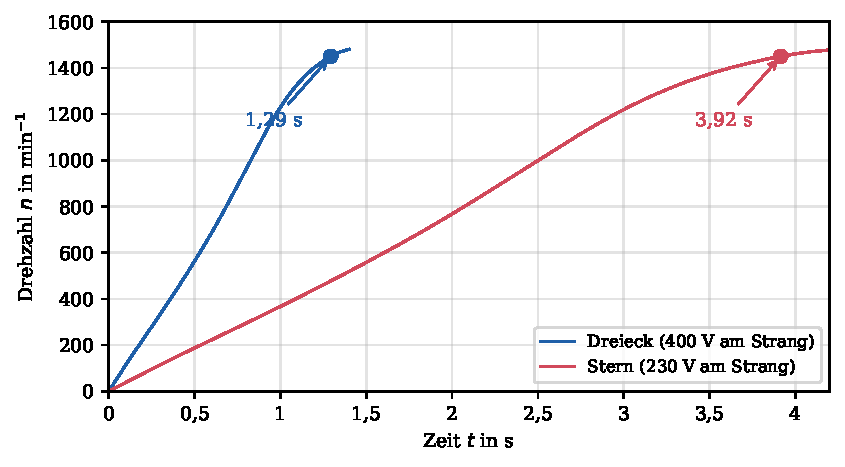
\includegraphics[width=0.8\textwidth]{v_hochlauf}
\caption{التسارع المحسوب (\dt{Dreieck} = مثلث، \dt{Stern} = نجمة)}
\end{figure}

% =====================================================================
\section{تجارب التشغيل: ماذا تُظهر الرسوم؟}
% =====================================================================
\textbf{كيف تقرأ الرسم:} كل رسم تشغيل فيه أربعة أجزاء فوق بعضها:
\begin{enumerate}
\item السرعة $n$،
\item التيار $I$،
\item الجهد $U$،
\item القدرة الفعالة $P$ والقدرة الردّية $Q$.
\end{enumerate}
المنطقة الرمادية هي فترة التبديل، حيث يكون المحرك بلا تيار لوقت قصير.

\subsection{التشغيل المباشر بالمثلث (الملف \datei{Stern-Dreieck\_direkt.csv})}
\begin{figure}[H]\centering
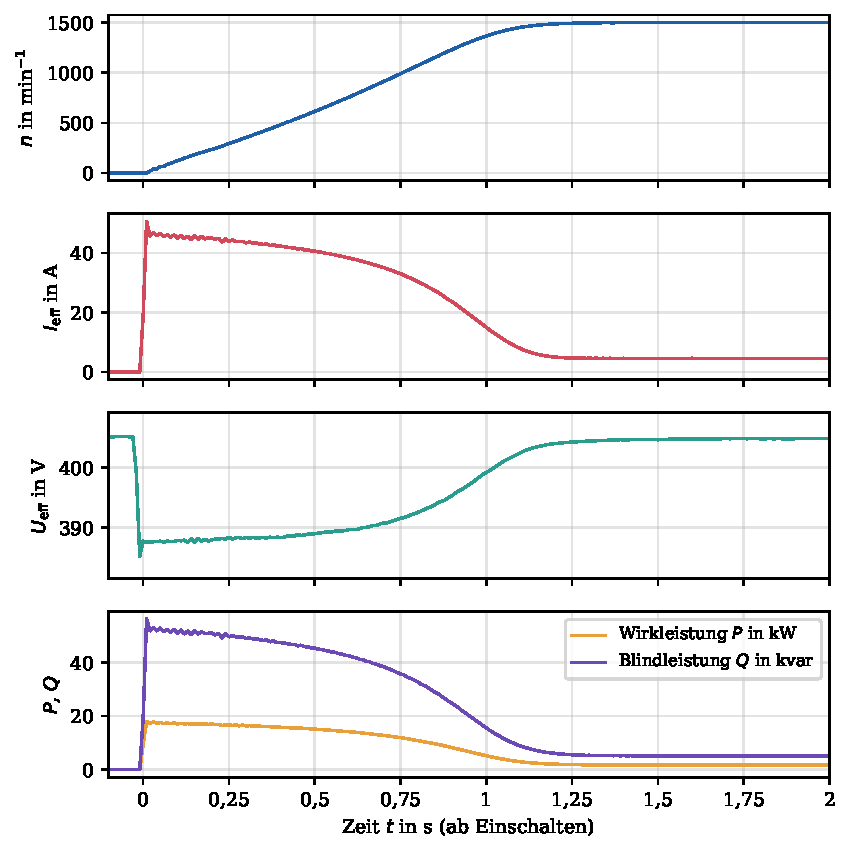
\includegraphics[width=0.72\textwidth]{a_direkt}
\end{figure}
\textbf{سير العملية:}
\begin{enumerate}
\item عند التوصيل يقفز التيار إلى حوالي \SI{50}{A}، وينخفض الجهد من \SI{405}{V} إلى \SI{388}{V}
      (\SI{\WdirektdU}{\percent}).
\item يبقى التيار مرتفعًا مدة طويلة، لأن الممانعة صغيرة حتى انزلاق الانقلاب.
\item ابتداءً من حوالي \SI{1000}{\per\minute} (عزم الانقلاب) ينخفض التيار بسرعة إلى تيار اللاحمل
      \SI{4,6}{A} ويعود الجهد.
\item بعد \SI{\Wdirekttneunacht}{s} ينتهي التسارع.
\end{enumerate}
\textbf{القدرات:}
\begin{itemize}
\item $Q\approx 3\cdot P$، أي $\cos\varphi\approx0{,}3$: تيار التشغيل أغلبه تيار ردّي.
\item في اللاحمل $P\approx\SI{1,75}{kW}$: وهي مفاقيد الحديد والاحتكاك والنحاس في اللاحمل.
      المحرك ليس عليه حمل.
\end{itemize}

\subsection{نجمة-مثلث مع تبديل مبكر جدًا}
\begin{figure}[H]\centering
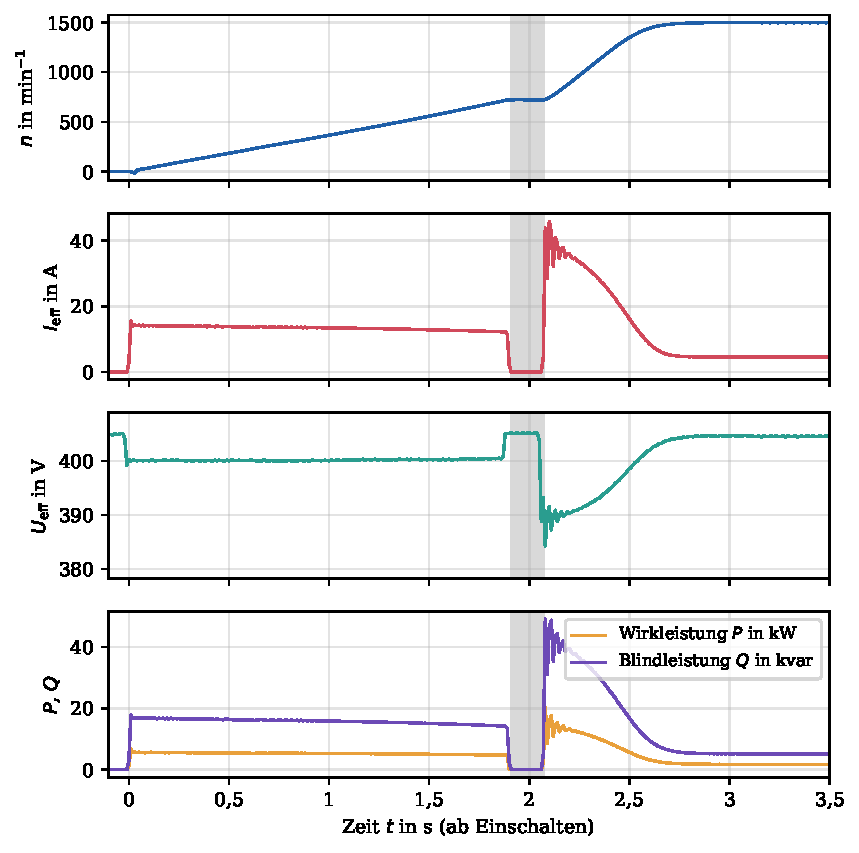
\includegraphics[width=0.72\textwidth]{a_frueh}
\end{figure}
\textbf{سير العملية:}
\begin{enumerate}
\item في النجمة يكون التيار حوالي \SI{15}{A} فقط، أي الثلث، والجهد لا ينخفض تقريبًا.
\item الآلة تتسارع ببطء ثلاث مرات أكثر.
\item يتم التبديل عند \SI{\Wfruehnum}{\per\minute} فقط، وهي بعيدة عن السرعة الاسمية: الانزلاق ما زال كبيرًا.
\item لذلك يعود في المثلث تقريبًا كامل تيار التشغيل: \SI{\WfruehIzwei}{A}،
      وينخفض الجهد حتى \SI{\WfruehUzwei}{V}.
\end{enumerate}
\textbf{الخلاصة:} الشبكة تتلقى رغم ذلك صدمة تيار كبيرة. توصيلة نجمة-مثلث لم تُفِد تقريبًا.
\begin{achtung}
حسب الدليل كان يجب أن يكون زمن التبديل \SI{0,5}{s}. لكن في بيانات القياس يحدث التبديل بعد حوالي
\SI{1,9}{s}. ربما ضُبطت قيمة أخرى يوم التجربة. تحقق من ملاحظاتك. في التقرير القيمة المقيسة من البيانات.
\end{achtung}

\subsection{نجمة-مثلث مع تبديل في الوقت الصحيح}
\begin{figure}[H]\centering
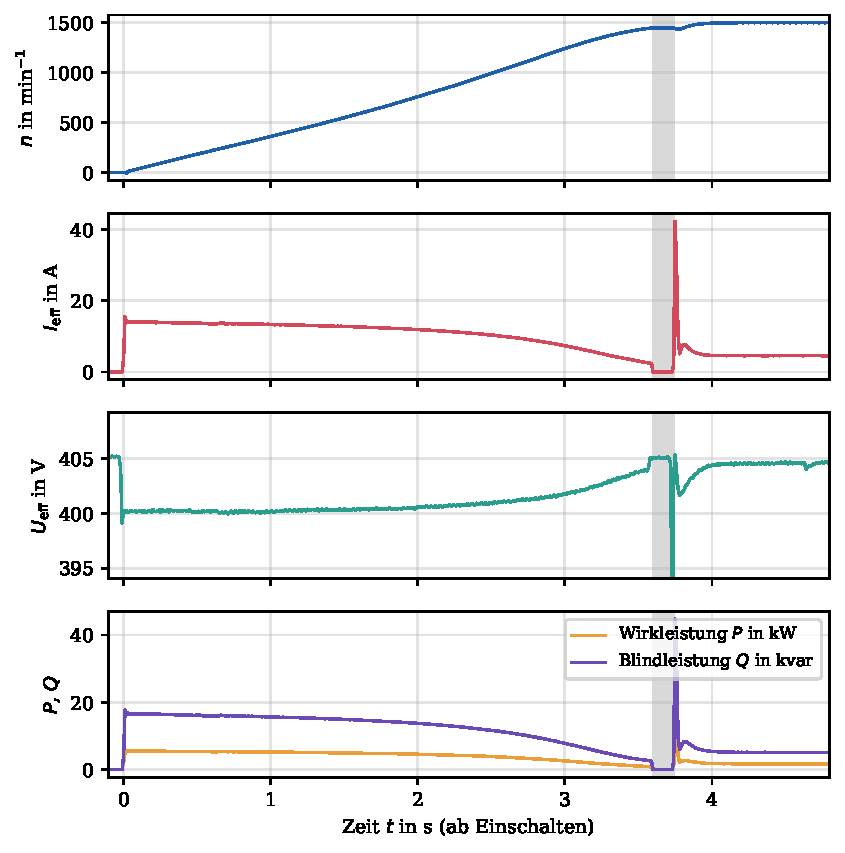
\includegraphics[width=0.72\textwidth]{a_richtig}
\end{figure}
\textbf{سير العملية:}
\begin{enumerate}
\item التبديل عند \SI{\Wrichtignum}{\per\minute} بعد \SI{\Wrichtigtum}{s}، وهذا يطابق الحساب.
\item كان التيار قد انخفض قبلها إلى حوالي \SI{2,5}{A}.
\item عند التبديل تظهر قمة قصيرة جدًا فقط (حوالي \SI{20}{ms}).
\end{enumerate}
\textbf{من أين تأتي هذه القمة أصلًا؟} أثناء الاستراحة القصيرة يبقى الدوّار ممغنطًا ويولّد جهدًا خاصًا به،
هو \emph{الجهد المتبقي} \de{Restspannung}. عند إعادة التوصيل لا يتطابق جهد الشبكة والجهد المتبقي تمامًا،
فيمر تيار موازنة قصير.

\subsection{نجمة-مثلث مع توصيل خاطئ}
\begin{figure}[H]\centering
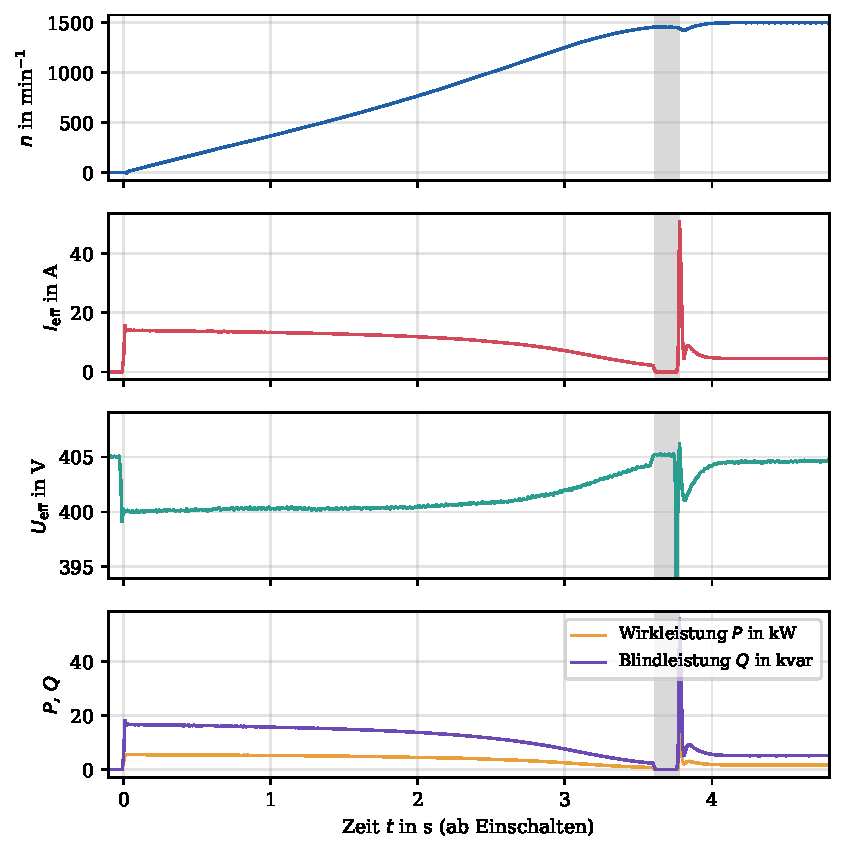
\includegraphics[width=0.72\textwidth]{a_falsch}
\end{figure}
\textbf{الفرق عن التوصيل الصحيح:} نفس سرعة التبديل، لكن
\begin{itemize}
\item قمة التيار أكبر (\SI{\WfalschIzwei}{A} بدل \SI{\WrichtigIzwei}{A})،
\item قمة القدرة الفعالة تقريبًا الضعف،
\item السرعة تنخفض لحظيًا بحوالي \SI{30}{\per\minute}.
\end{itemize}
\begin{einfach}
\begin{itemize}
\item عند التبديل من نجمة إلى مثلث يدور جهد كل ملف بزاوية \SI{30}{\degree}.
\item اتجاه هذه القفزة (للأمام أو للخلف) يعتمد على طريقة توصيل أطراف الملفات
      \dt{U2, V2, W2} بالخطوط \dt{L1, L2, L3}.
\item مع التوصيل الصحيح يكون جهد الشبكة الجديد قريبًا من الجهد المتبقي للدوّار، فتكون الصدمة صغيرة.
\item مع التوصيل الخاطئ تكون الزاوية بينهما أكبر، فيكبر تيار الموازنة، بل ويكبح المحرك لحظة
      (ولهذا تنخفض السرعة).
\end{itemize}
\end{einfach}
\begin{achtung}
هذا هو التفسير المعتاد. أما ما كان خاطئًا بالضبط في التوصيل يوم التجربة فلا تعرفه إلا من ملاحظاتك
أو من المشرف. اسأل إن لم يكن واضحًا.
\end{achtung}

\subsection{عزم التسارع من القياس}
\textbf{الطريقة:}
\begin{enumerate}
\item نشتق السرعة بالنسبة للزمن: $\mathrm dn/\mathrm dt$.
\item نضرب في $J$ و $2\pi$: $M_B = J\cdot2\pi\cdot\mathrm dn/\mathrm dt$.
\end{enumerate}
لأن السرعة المقيسة فيها تشويش (القيم تقفز بمقدار $\pm\SI{1}{\per\minute}$) يجب تنعيمها أولًا.
استخدمت \emph{مرشّح سافيتسكي-غولاي} \de{Savitzky-Golay-Filter}، وهو يضع قطعًا مكافئًا (بارابولا) عبر
نقاط القياس على أجزاء.

\textbf{بديل في إكسل:} خارج قسمة الفروق $(n_{i+5}-n_{i-5})/(t_{i+5}-t_{i-5})$ على عدة نقاط، وهذا ينعّم أيضًا.
\begin{figure}[H]\centering
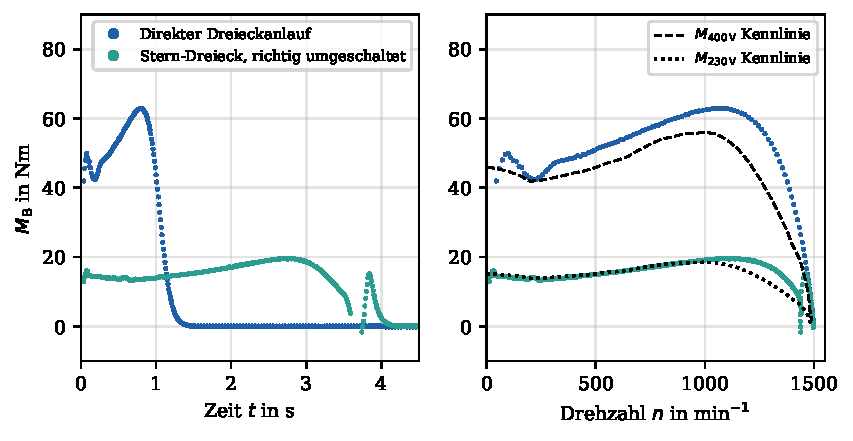
\includegraphics[width=0.9\textwidth]{a_moment}
\end{figure}
\textbf{النتيجة:}
\begin{itemize}
\item شكل المنحنى يظهر في القياس: السَّرج، نقطة الانقلاب، الانخفاض.
\item في النجمة يتطابق القياس والحساب تقريبًا تمامًا.
\item في المثلث العزم المقيس أكبر بحوالي \SI{8}{\percent} من المنحنى.
      لذلك زمن التسارع المقيس أقصر من المحسوب
      (\SI{\Wdirektteinsvierfuenfnull}{s} بدل \SI{\WtHDB}{s}).
\end{itemize}

\begin{merke}
أسباب الاختلاف بين القياس والحساب:
\begin{itemize}
\item منحنى الشركة المصنعة له تفاوتات (سماحيات).
\item الجهد كان \SI{405}{V} بدل \SI{400}{V}. وبما أن $M\sim U^2$ فهذا يعطي $+\SI{2,5}{\percent}$ عزمًا.
\item المنحنى قُرئ من صورة.
\item قيمة $J$ في الدليل أكبر قليلًا.
\item من الصعب تحديد اللحظة التي «ينتهي» فيها التسارع بدقة.
\end{itemize}
\end{merke}

\subsection{الطاقة – ملاحظة إضافية جميلة}
\begin{itemize}
\item في النهاية تختزن الحذافة $E = \frac12J\omega^2\approx\SI{4,6}{kJ}$.
\item لكن الطاقة المأخوذة من الشبكة كانت حوالي \SIrange{14,5}{15,8}{kJ}.
\item \textbf{السبب:} عند تسريع محرك لاتزامني بلا حمل يتحوّل في الدوّار إلى حرارة مقدار من الطاقة
      يساوي ما يُخزَّن في الحذافة. ويضاف إلى ذلك مفاقيد الجزء الثابت والحديد.
\item إذن توصيلة نجمة-مثلث \emph{لا توفّر طاقة}. هي فقط توزّع التيار على زمن أطول وتتجنب القمم العالية.
\end{itemize}

% =====================================================================
\section{تجارب الكبح: ماذا تُظهر الرسوم؟}
% =====================================================================
\textbf{نقطة البداية:}
\begin{itemize}
\item المحرك موصول بمغيّر تردد \de{Frequenzumrichter, FU}، السرعة حوالي \SI{1800}{\per\minute}
      (\SI{60}{Hz})، مع قرص ألمنيوم.
\item $t=0$ هي لحظة أمر الكبح.
\item الطاقة في القرص: $E_\mathrm{kin} = \frac12\cdot0{,}1277\cdot(2\pi\cdot30)^2\approx\SI{2270}{J}$.
\item عزم الكبح: $M_\mathrm{Br} = -J\cdot2\pi\cdot\mathrm dn/\mathrm dt$.
\end{itemize}

\subsection{مغيّر التردد في 4 أجزاء}
\begin{enumerate}
\item \textbf{المقوّم} \de{Gleichrichter} (ثنائيات/دايودات): يحوّل جهد الشبكة المتناوب إلى جهد مستمر.
  يستطيع فقط \emph{أخذ} الطاقة، و\emph{لا يستطيع إرجاعها إلى الشبكة}.
\item \textbf{الدائرة الوسيطة} \de{Zwischenkreis} (مكثّف): حوالي $\sqrt2\cdot\SI{400}{V}\approx\SI{565}{V}$،
  والمقيس \SI{580}{V}.
\item \textbf{مقطّع الكبح} \de{Brems-Chopper} مع مقاومة الكبح: ترانزستور يوصل المقاومة عندما يصبح جهد
  الدائرة الوسيطة مرتفعًا جدًا.
\item \textbf{العاكس} \de{Wechselrichter} (\dt{IGBT}): يولّد تيارًا ثلاثي الطور بأي تردد.
\end{enumerate}
\begin{merke}
أهم شيء لكل أسئلة الكبح: مقوّم الدايودات طريق في اتجاه واحد. طاقة الكبح لا تستطيع الرجوع إلى الشبكة،
فيجب تحويلها إلى حرارة: في المحرك (كبح التيار المستمر)، أو في مقاومة الكبح، أو في فرامل الاحتكاك.
\end{merke}

\subsection{نظرة عامة}
\begin{figure}[H]\centering
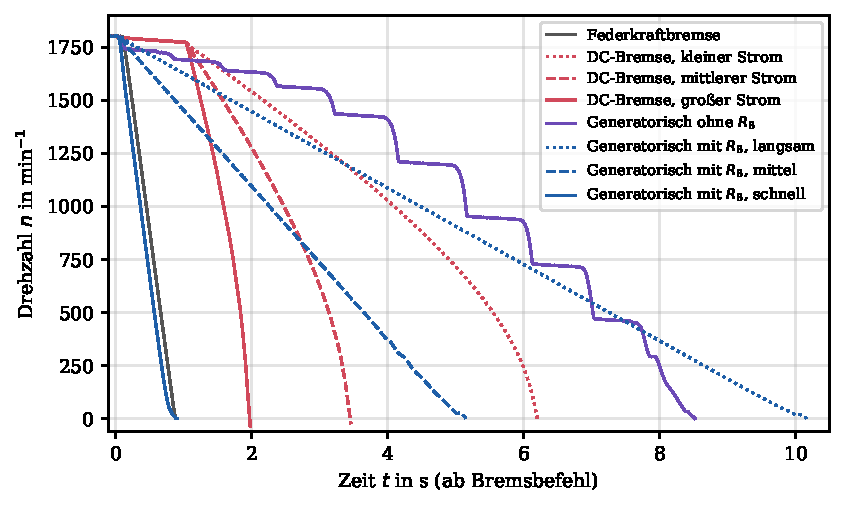
\includegraphics[width=0.85\textwidth]{b_vergleich_n}
\end{figure}

\subsection{فرامل النابض}
\textbf{طريقة العمل:}
\begin{itemize}
\item نابض يضغط بطانات الفرامل معًا.
\item مغناطيس كهربائي يُبقي الفرامل مفتوحة، أي «محرَّرة» \de{gelüftet}.
\item ينقطع التيار $\Leftarrow$ يترك المغناطيس $\Leftarrow$ النابض يكبح.
\end{itemize}
\textbf{القياس:}
\begin{itemize}
\item تأخير حوالي \SI{\Wfederts}{s} (زمن الانطباق: يجب أن يختفي المجال المغناطيسي أولًا)،
\item بعدها تنخفض السرعة \textbf{خطيًا}، أي أن العزم ثابت: حوالي \SI{\WfederMmit}{Nm}،
\item التوقف بعد \SI{\WfedertB}{s}.
\end{itemize}
\textbf{لماذا العزم ثابت؟} الاحتكاك الجاف (احتكاك كولوم) لا يعتمد على السرعة:
قوة الاحتكاك $=\mu\times$ قوة النابض.

\subsection{الكبح بالتيار المستمر \dt{(DC-Bremse)}}
\textbf{طريقة العمل:}
\begin{itemize}
\item يرسل مغيّر التردد تيارًا مستمرًا في ملف الجزء الثابت، فينشأ مجال مغناطيسي \emph{ثابت لا يدور}.
\item الدوّار الدائر يقطع هذا المجال، فيُحَث فيه تيار وينشأ عزم كبح، مثل فرامل التيارات الدوامية.
\end{itemize}
\textbf{القياس:}
\begin{itemize}
\item أولًا لا يحدث شيء لمدة حوالي \SI{1}{s}: ينتظر مغيّر التردد حتى يختفي الجهد المتبقي للمحرك
      (زمن إزالة المغنطة). وإلا لمرّ تيار قصر.
\item بعدها يتم الكبح بـ \SI{\WdclIdcB}{A} أو \SI{\WdcmIdcB}{A} أو \SI{\WdcsIdcB}{A}.
\item ينخفض زمن الكبح من \SI{\WdcltnachI}{s} إلى \SI{\WdcmtnachI}{s} ثم إلى \SI{\WdcstnachI}{s}.
\end{itemize}
\begin{figure}[H]\centering
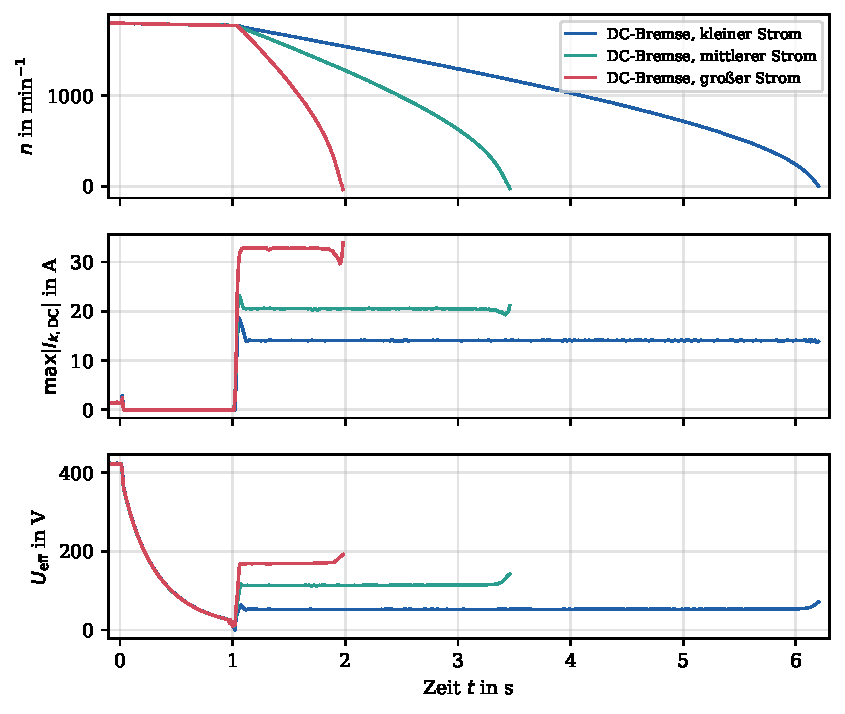
\includegraphics[width=0.72\textwidth]{b_dc}
\end{figure}
\textbf{ثلاثة أشياء يجب أن تستطيع شرحها:}
\begin{enumerate}
\item \textbf{العزم $\sim I^2$:} المجال $\sim I$، وتيار الدوّار المُحَث أيضًا $\sim I$، إذن العزم $\sim I^2$.
  المقيس: التيار $\times1{,}45$ $\Leftarrow$ العزم $\times2{,}1$، والتيار $\times2{,}33$ $\Leftarrow$
  العزم $\times5{,}5$. مطابق!
\item \textbf{العزم يكبر قرب النهاية} (المنحنى يصبح أشد انحدارًا): عند السرعة العالية يكون تردد الدوّار
  عاليًا، فيكون الدوّار حثّيًا بقوة ويكون التيار «في غير مكانه» بالنسبة للمجال. عند السرعة الصغيرة يكون
  الوضع أفضل. لذلك تكون القيمة العظمى قبيل التوقف، مثل منحنى المحرك لكن معكوسًا.
\item \textbf{لا يوجد عزم إمساك:} عند $n=0$ لا يُحَث شيء، فلا يوجد عزم. حِمل معلّق (رافعة) سينزل ببطء.
  إضافة إلى ذلك تتحول كل الطاقة إلى حرارة \emph{داخل المحرك}، فيسخن.
\end{enumerate}

\subsection{الكبح التوليدي بدون مقاومة كبح}
\textbf{طريقة العمل:} يُخفّض مغيّر التردد التردد، فتدور الآلة أسرع من المجال ($s<0$) وتصبح مولّدًا.
تذهب الطاقة إلى الدائرة الوسيطة.

\textbf{القياس والتفسير:}
\begin{itemize}
\item يرتفع $U_\mathrm{ZK}$ من \SI{580}{V} حتى \SI{\WgenohneUzkmax}{V}.
\item عند الجهد الزائد يوقف مغيّر التردد النبضات، فيصبح التيار صفرًا ويدور المحرك حرًّا.
\item عندما ينخفض $U_\mathrm{ZK}$ من جديد تأتي نبضة كبح قصيرة، وتتكرر العملية.
\item النتيجة: تنخفض السرعة على شكل درجات، ولا يتوقف المحرك إلا بعد \SI{\WgenohnetB}{s}.
\end{itemize}
\begin{figure}[H]\centering
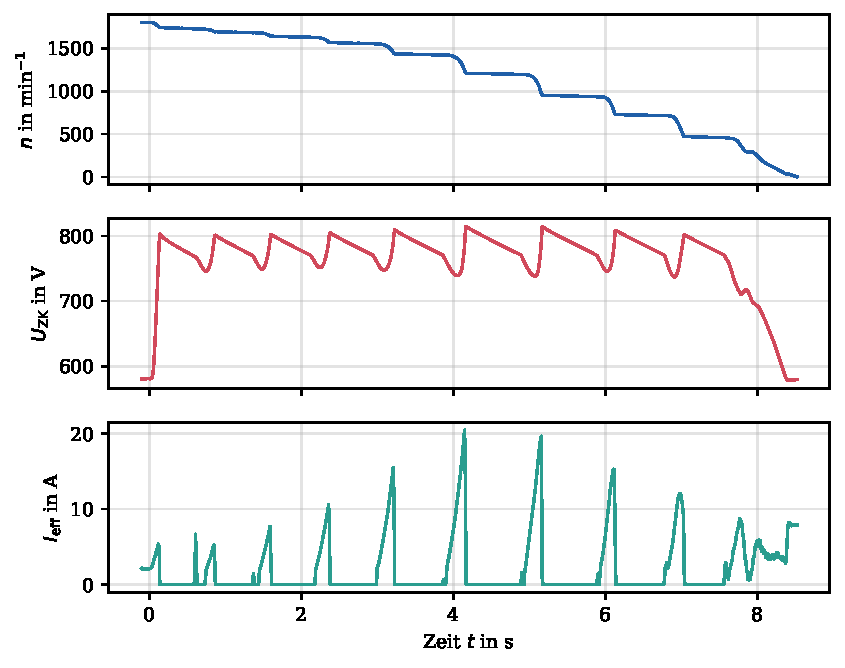
\includegraphics[width=0.72\textwidth]{b_gen0}
\end{figure}

\subsection{الكبح التوليدي مع مقاومة كبح}
\textbf{القياس:}
\begin{itemize}
\item يحدّ مقطّع الكبح الجهد $U_\mathrm{ZK}$ عند حوالي \SI{720}{V}.
\item يتبع المحرك المنحدر \de{Rampe} بدقة: تنخفض السرعة خطيًا ويكون العزم ثابتًا.
\item أزمنة الكبح: بطيء \SI{\WgenltB}{s}، متوسط \SI{\WgenmtB}{s}، سريع \SI{\WgenstB}{s}.
\item في الحالة السريعة تستقبل المقاومة حتى \SI{7,8}{kW}. وإجمالًا تذهب إليها حوالي \SI{\WgensErb}{J}،
      أي \SI{\WgensErbAnteil}{\percent} من الطاقة الحركية. الباقي مفاقيد في المحرك ومغيّر التردد.
\item في المنحدر البطيء نادرًا ما يعمل المقطّع، لأن مفاقيد المحرك ومغيّر التردد تكفي تقريبًا لقدرة الكبح الصغيرة.
\end{itemize}
\textbf{تقدير مقاومة الكبح:} المقطّع يمرّر التيار على شكل نبضات.
\begin{itemize}
\item نسبة التشغيل: $D = (I_\mathrm{mittel}/I_\mathrm{eff})^2$.
\item التيار في حالة التشغيل: $I_\mathrm{ein} = I_\mathrm{mittel}/D$.
\item المقاومة: $R = U_\mathrm{ZK}/I_\mathrm{ein}\approx\SI{\WRb}{\ohm}$.
\end{itemize}
\begin{figure}[H]\centering
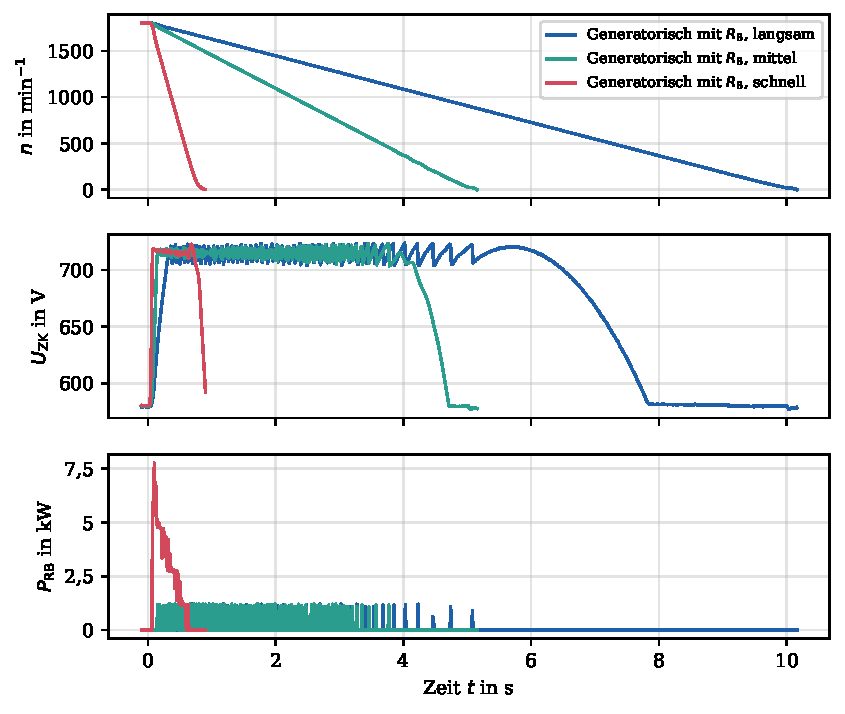
\includegraphics[width=0.72\textwidth]{b_gen}
\end{figure}

\subsection{مقارنة عزوم الكبح}
\begin{figure}[H]\centering
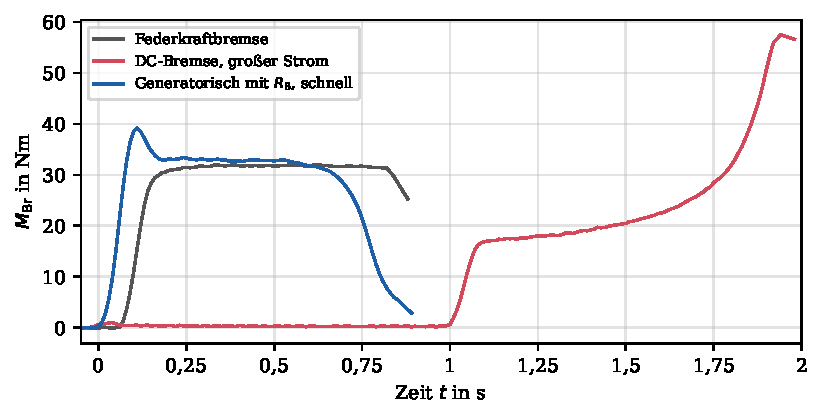
\includegraphics[width=0.8\textwidth]{b_moment_zoom}
\end{figure}
\begin{center}
\begin{tabular}{@{}lccc@{}}
\toprule
الطريقة & شكل العزم & عزم إمساك؟ & أين تتحول الطاقة إلى حرارة؟\\
\midrule
فرامل النابض & ثابت & نعم & بطانات الفرامل\\
كبح التيار المستمر & يزداد نحو التوقف & لا & المحرك (الدوّار)\\
توليدي بدون $R_B$ & نبضات قصيرة فقط & لا & المفاقيد، المكثّف\\
توليدي مع $R_B$ & ثابت (منحدر) & لا & مقاومة الكبح\\
\bottomrule
\end{tabular}
\end{center}

% =====================================================================
\section{أسئلة الدليل – إجابات بكلماتك}
% =====================================================================
\begin{frage}{من أين يأتي انخفاض الجهد، وكيف يمكن تقليله؟}
\textbf{السبب:}
\begin{itemize}
\item تيار التشغيل الكبير يمرّ عبر الممانعة الداخلية للشبكة (المحول والكابلات).
\item هذا التيار ردّي تقريبًا بالكامل، والمحول حثّي في الأساس.
\item لذلك يُنقص هبوط الجهد جهد الشبكة مباشرة.
\end{itemize}
\textbf{العلاج:}
\begin{itemize}
\item نجمة-مثلث (مضبوطة بشكل صحيح)، بادئ ناعم \de{Sanftanlasser}، مغيّر تردد، محول بدء.
\item محول أقوى بقيمة $u_k$ صغيرة، كابلات أسمك أو أقصر.
\end{itemize}
\end{frage}

\begin{frage}{مقارنة زمن التسارع المحسوب مع المقيس}
\begin{itemize}
\item المثلث: محسوب \SI{\WtHDB}{s}، مقيس \SI{\Wdirektteinsvierfuenfnull}{s}.
\item النجمة: محسوب حوالي \SI{\WtHYum}{s}، مقيس \SI{\Wrichtigtum}{s} (حتى \SI{1443}{\per\minute}).
\end{itemize}
القياس أسرع قليلًا لأن الآلة الحقيقية لها عزم أكبر (التفاوتات، \SI{405}{V}، خطأ القراءة).
أما شكل المنحنى فمطابق جدًا.
\end{frage}

\begin{frage}{احسب عزم التسارع وقارنه بالتحضير}
\begin{itemize}
\item المعادلة: $M = J\cdot2\pi\cdot\mathrm dn/\mathrm dt$ مع $J = \SI{0,3711}{kg.m^2}$.
\item النتيجة: الشكل يشبه المنحنى. المتوسط في المثلث \SI{\WdirektMBmittel}{Nm}
      (المنحنى \SI{\WMkennDmittel}{Nm})، وفي النجمة \SI{\WrichtigMBmittel}{Nm}
      (المنحنى \SI{\WMkennYmittel}{Nm}).
\end{itemize}
\end{frage}

\begin{frage}{لماذا الكبح التوليدي بدون مقاومة أبطأ بكثير؟}
\begin{itemize}
\item الطاقة لا تستطيع الرجوع إلى الشبكة، لأن مقوّم الدايودات طريق في اتجاه واحد.
\item بدون مقاومة لا يوجد مكان تذهب إليه الطاقة.
\item يرتفع $U_\mathrm{ZK}$ حتى حد الجهد الزائد، فيقطع مغيّر التردد الكبح.
\item مع المقاومة تتحول الطاقة إلى حرارة ويُحترم المنحدر: \SI{0,87}{s} بدل \SI{8,5}{s}.
\end{itemize}
\end{frage}

\begin{frage}{أي طريقة تصلح للإيقاف الطارئ \dt{(Not-Halt)}؟}
\textbf{فرامل النابض}، لأنها
\begin{itemize}
\item تكبح \emph{بدون تيار} (آمنة عند العطل، مبدأ تيار السكون \de{Ruhestromprinzip})،
\item تعمل حتى عند انقطاع الشبكة أو عطل مغيّر التردد،
\item \emph{تمسك} الحمل عند التوقف.
\end{itemize}
كل الطرق الكهربائية تحتاج إلى الشبكة وإلى مغيّر التردد. في التطبيق العملي نجمع الطرق:
أولًا كبح توليدي (يحافظ على البطانات)، ثم تنطبق فرامل النابض (فئة الإيقاف 1).
\end{frage}

% =====================================================================
\section{أسئلة محتملة للامتحان الشفهي \dt{(Testat)}}
% =====================================================================
\begin{enumerate}[label=\textbf{س\arabic*:},leftmargin=2.4em]
\item \emph{لماذا يكون تيار التشغيل من 5 إلى 8 أضعاف التيار الاسمي؟}\\
  عند $s=1$ يكون المحرك مثل محول مقصور، ولا يحدّ التيار إلا ممانعة القصر الصغيرة.
\item \emph{لماذا لا ينخفض التيار بقوة إلا بعد عزم الانقلاب؟}\\
  لأن مقاومة الدوّار $R_2'/s$ لا تكبر إلا عند الانزلاق الصغير. قبل ذلك تبقى الممانعة صغيرة.
\item \emph{بأي معامل ينخفض التيار والعزم في النجمة؟}\\
  كلاهما إلى الثلث. السبب: جهد الملف $/\sqrt3$، و $M\sim U^2$، وتيار الخط $\sqrt3\cdot\sqrt3 = 3$.
\item \emph{متى لا يجوز استخدام نجمة-مثلث؟}\\
  عندما يكون عزم الحمل عند البدء أكبر من ثلث عزم المحرك، مثل السيور الثقيلة أو الرافعات.
  الأفضل حينها مغيّر تردد.
\item \emph{ماذا يحدث عند التبديل المبكر؟}\\
  صدمة تيار ثانية، تقريبًا مثل التشغيل المباشر.
\item \emph{ماذا يحدث إذا لم يصل المحرك إلى السرعة في النجمة؟}\\
  يبقى عالقًا عند السرعة التي يكون فيها $M_{230} = M_\mathrm{Last}$، ويسحب تيارًا عاليًا مدة طويلة
  فيسخن بشكل زائد.
\item \emph{كيف نحسب العزم من السرعة؟}\\
  $M = J\cdot2\pi\cdot\mathrm dn/\mathrm dt$، مع $n$ بوحدة \si{\per\second}.
\item \emph{كم يساوي $J$ لقرص مصمت؟}\\
  $\frac12 m r^2$. انتبه: نصف القطر وليس القطر!
\item \emph{لماذا لا يوجد عزم إمساك في كبح التيار المستمر؟}\\
  بدون حركة لا يُحَث شيء.
\item \emph{أين تذهب الطاقة في كبح التيار المستمر؟}\\
  إلى المحرك (الدوّار والجزء الثابت)، فيسخن.
\item \emph{لماذا يرتفع $U_\mathrm{ZK}$ في الكبح التوليدي؟}\\
  الطاقة تذهب إلى المكثّف، ومقوّم الدايودات لا يستطيع إرجاعها إلى الشبكة.
\item \emph{ما هو مقطّع الكبح؟}\\
  ترانزستور يوصل مقاومة الكبح بالدائرة الوسيطة عندما يتجاوز الجهد حدًّا معيّنًا.
\item \emph{كيف يمكن الاستفادة من طاقة الكبح بدل تحويلها إلى حرارة؟}\\
  بمغيّر تردد قادر على إرجاع الطاقة \dt{(Active Front End)} أو بدائرة وسيطة مشتركة لعدة محركات.
\item \emph{لماذا فرامل النابض آمنة عند العطل؟}\\
  النابض هو الذي يكبح، والتيار فقط \emph{يحرّر} الفرامل. إذا انقطع التيار تعمل الفرامل.
\item \emph{لماذا يحتاج كبح التيار المستمر إلى زمن انتظار قبل حقن التيار؟}\\
  المحرك ما زال ممغنطًا ويولّد جهدًا متبقيًا. لو حقن مغيّر التردد التيار فورًا لحدثت تيارات زائدة.
\end{enumerate}

% =====================================================================
\section{ملخّص المعادلات}
% =====================================================================
\begin{center}
\renewcommand{\arraystretch}{1.5}
\begin{tabular}{@{}ll@{}}
\toprule
السرعة التزامنية & $n_s = f/p$\\
الانزلاق & $s = (n_s-n)/n_s$\\
القدرة والعزم & $P = M\cdot\omega = M\cdot2\pi n$\\
العزم والجهد & $M\sim U^2$, \quad $M_{230} = \frac13M_{400}$\\
معادلة الحركة & $J\,\mathrm d\omega/\mathrm dt = M_\mathrm{Mot} - M_\mathrm{Last}$\\
خطوة الزمن & $\Delta t = 2\pi J\Delta n/M$\\
عزم القصور (قرص مصمت) & $J = \frac12 m r^2$\\
الطاقة الحركية & $E = \frac12 J\omega^2$\\
هبوط الجهد (كاب) & $\Delta U\approx I(R_k\cos\varphi + X_k\sin\varphi)$\\
معامل القدرة & $\cos\varphi = P/\sqrt{P^2+Q^2}$\\
عزم كبح التيار المستمر & $M_\mathrm{Br}\sim I_\mathrm{DC}^2$\\
\bottomrule
\end{tabular}
\end{center}

% =====================================================================
\section{قاموس ألماني – عربي (كلمات الرسوم البيانية)}
\label{sec:lexique}
% =====================================================================
\begin{center}
\begin{tabular}{@{}p{0.45\textwidth}p{0.45\textwidth}@{}}
\toprule
الألمانية & العربية\\
\midrule
\dt{Drehzahl $n$} & سرعة الدوران\\
\dt{Zeit $t$ (ab Einschalten / ab Bremsbefehl)} & الزمن (من لحظة التشغيل / من أمر الكبح)\\
\dt{Moment, Drehmoment $M$} & العزم\\
\dt{Wirkleistung / Blindleistung} & القدرة الفعالة / القدرة الردّية\\
\dt{Strom / Spannung} & التيار / الجهد\\
\dt{Stern / Dreieck} & نجمة / مثلث\\
\dt{Anlauf / Hochlauf} & التشغيل / التسارع حتى السرعة\\
\dt{umschalten, Umschaltpause} & التبديل، فترة التبديل\\
\dt{zu früh / richtig / falsch verdrahtet} & مبكر جدًا / صحيح / موصول خطأ\\
\dt{Kennlinie, Rechnung} & المنحنى المميز، الحساب\\
\dt{Zwischenkreisspannung $U_\mathrm{ZK}$} & جهد الدائرة الوسيطة\\
\dt{Bremswiderstand $R_B$} & مقاومة الكبح\\
\dt{Federkraftbremse} & فرامل النابض\\
\dt{DC-Bremse, kleiner/mittlerer/großer Strom} & كبح بالتيار المستمر، تيار صغير/متوسط/كبير\\
\dt{Generatorisch, langsam/mittel/schnell} & توليدي، بطيء/متوسط/سريع\\
\dt{Kippmoment / Sattelmoment / Anzugsmoment} & عزم الانقلاب / عزم السَّرج / عزم البدء\\
\dt{Schlupf} & الانزلاق\\
\dt{Frequenzumrichter (FU)} & مغيّر التردد\\
\dt{Schwungmasse / Schwungscheibe} & الحذافة\\
\bottomrule
\end{tabular}
\end{center}

% =====================================================================
\section{ملاحظات مهمة حول ملفاتك}
% =====================================================================
\begin{itemize}
\item \textbf{ملفات لم تُستخدم:} الملفات \datei{F\_Kennline\_Dreick.csv} و
  \datei{F\_Kennline\_Stern.csv} و \datei{Messung\_f87Hz\_*.csv} لا تنتمي إلى التجربة 9.
  إنها منحنيات تردد أو تشغيل على \SI{87}{Hz}، وغالبًا من تجربة أخرى، لذلك ليست في التقرير.
\item \textbf{أسماء الملفات:} الملف \datei{Stern-Dreieck\_direkt.csv} هو \emph{التشغيل المباشر بالمثلث}
  (يظهر ذلك من تيار التشغيل البالغ \SI{50}{A}).
\item \textbf{قبل التسليم:} املأ صفحة الغلاف (الأسماء، أرقام التسجيل، المجموعة، التاريخ).
  وتحقق أيضًا من زمن التبديل «المبكر» (\SI{0,5}{s} حسب الدليل، و\SI{1,9}{s} في البيانات).
\item \textbf{التعديل:} إذا أردت تغيير قيم، عدّل البيانات أو السكربت \datei{auswertung/auswertung.py}،
  ثم شغّله \dt{(\texttt{python3 auswertung.py})} وأعد ترجمة التقرير. كل الأرقام في النص تتحدث تلقائيًا.
\end{itemize}
\end{document}
